% ACM SIGMETRICS 2027 -- Fall cycle submission (double anonymous)
% Class line is mandated verbatim by the official CFP:
%   \documentclass[acmsmall, screen, review]{acmart}
% Generated by docs/paper/submission/scripts/md2tex.py from the frozen
% manuscript d137a7d. Do not edit main.tex by hand -- edit the frozen
% Markdown (which is closed) or the converter, and regenerate.
\documentclass[acmsmall, screen, review, anonymous]{acmart}

\usepackage{booktabs}
\usepackage{graphicx}
\usepackage{tabularx}
% wrapping, left-aligned variable-width column for wide text columns
\newcolumntype{L}{>{\raggedright\arraybackslash}X}
% Long machine identifiers (e.g. software_visible_completion_observation_cycles)
% cannot break by default and overflow the text block. Allow hyphenation inside
% \texttt and give TeX a little emergency stretch. Typesetting only.
\usepackage[htt]{hyphenat}
\emergencystretch=2em

% Double-anonymous: no author, affiliation, funding or acknowledgement data is
% present anywhere in this file. See ANONYMITY_AUDIT.md.
\settopmatter{printacmref=false}
\acmConference[SIGMETRICS '27]{ACM SIGMETRICS}{2027}{}
\acmISBN{}
\acmDOI{}
\copyrightyear{2027}
\acmYear{2027}
\setcopyright{none}

\begin{document}

\title{Characterizing Arm Ethos-U NPU Configurations: Simulated Scaling, Hardware Validation, and an Operator-Level Mechanism Study}

\begin{abstract}
 Embedded ML deployment on Arm Ethos-U NPUs forces configuration choices --- NPU generation, MAC count, memory mode, host subsystem --- long before hardware exists, and those choices are made from compiler estimates and cycle-model simulation. We characterize what those tools actually support. Across a 133-cell capability universe we identify 74 executable, timing-adapter-enabled cells and measure them under a byte-reproducible provenance chain (222 samples), validate one configuration on physical Corstone-320 / Ethos-U85 hardware (21 samples), and decompose the single configuration transition where more MAC capacity measured \emph{slower}.  Three primary findings follow. \textbf{Scaling is workload-dependent and mostly sub-linear}: of 53 adjacent MAC transitions, 28 retain at least 75 \% efficiency and 23 fall between 50 \% and 75 \%, and saturation appears in only one of 21 ladders within the tested range. \textbf{One boundary is non-monotonic}: Ethos-U85 at 256 $\rightarrow$ 512 MACs makes \texttt{rnnoise} slower, and direct operation-group profiling shows the +19,000-cycle reversal is \emph{distributed} over ten operation groups rather than caused by any single structural change --- the same groups regress under every memory configuration tested, while a compiler-visible ublock change accompanies roughly 95 \% of operations in every direction class and therefore does not discriminate. \textbf{Compiler estimates preserve structure better than magnitude}: Vela matches the simulated saturation classification and speedup ordering in 19 of 20 ladders while per-step agreement varies widely.  Two results validate these findings rather than extending them. \textbf{Structural conclusions transfer better than labels}: in a same-artifact study across supported Corstone FVPs, workload ranking, scaling direction, saturation and normalized ordering are preserved, whereas threshold-based efficiency classes are more sensitive to timing-model configuration; on hardware, workload ordering is preserved exactly at the one measurable configuration.  We do not compare absolute cycles across generations, simulators or hardware, and we do not attribute the non-monotonicity to a single architectural or compiler factor; both remain outside what this evidence can separate. 

\end{abstract}
\maketitle
\section{Introduction}\label{sec:1}
Embedded ML deployment on Arm Ethos-U NPUs requires choosing among NPU generations, MAC configurations, memory modes, and host subsystems --- usually before any hardware exists. Practitioners make those choices from compiler estimates and cycle-model simulation, then discover on hardware what the estimates did not carry.

\textbf{Thesis.} Increasing MAC capacity does not yield proportional performance gains: scaling behaviour is workload-dependent and can become non-monotonic; where it does become non-monotonic, that transition is shaped by heterogeneous operation-level and memory/compiler interactions rather than by any single structural change; and the structural conclusions drawn from simulation transfer across the tested platform and timing conditions, whereas threshold-based labels proved sensitive to timing-model configuration and raw cross-platform cycles are not comparable at all.

We ask:

\begin{itemize}
  \item \textbf{RQ1} --- How do normalized scaling behaviour, workload ordering, and deployability differ across the supported Corstone/Ethos-U configurations? \emph{(Deliberately not ``which generation is faster'': Section~\ref{sec:3.3} sets out why absolute cross-generation cycle comparison is not admissible on this stack, and no result in this paper depends on one.)}
  \item \textbf{RQ2} --- How does performance scale with MAC configuration, and where does scaling saturate?
  \item \textbf{RQ3} --- To what extent do qualitative trends observed for Corstone-320 / Ethos-U85 in simulation reproduce on physical MPS4/FI101 hardware?
  \item \textbf{RQ4} --- For the one configuration transition where more hardware measured \emph{slower} --- Ethos-U85, 256 $\rightarrow$ 512 MACs --- what operator-level behaviour produces that whole-model non-monotonicity, and how robust is it to memory configuration?
\end{itemize}
\textbf{Primary contributions.}

\begin{enumerate}
  \item \textbf{A systematic MAC-scaling characterization} over a 133-cell capability universe and a 74-cell formal simulated sweep (222 samples) with byte-level artifact provenance, in which \textbf{executability is reported as a first-class result} rather than as missing data: all 133 cells compile and 6 cannot run.
  \item \textbf{An operator-level mechanism study of a non-monotonic boundary.} Using a post-compilation instrumentation path built and qualified for this purpose, we show the Ethos-U85 256 $\rightarrow$ 512 reversal is distributed across operation groups, recurs in the same groups under every tested memory configuration, and is not discriminated by any single compiler-visible transition.
  \item \textbf{A characterization of compiler cost estimates against simulation}, separating what Vela's performance model predicts well (saturation classification, speedup ordering) from what it does not (individual MAC-step magnitude).
\end{enumerate}
\textbf{Validation and supporting results.}

\begin{enumerate}
  \item \textbf{Physical-board ordering validation} on Corstone-320 / Ethos-U85 (21 formal samples), reporting ranking preservation and relative-cost shape, with absolute simulation-versus-hardware comparison refused by construction.
  \item \textbf{Platform-sensitivity robustness.} A same-artifact study across supported Corstone FVPs establishes which structural metrics survive a change of host platform and which do not.
  \item \textbf{Instrumentation qualification}, including a cross-backend bridge that bounds what per-layer numbers from two different instrumentation methods may be used for.
\end{enumerate}
Alongside these we report measurement-methodology results that generalize beyond this study: a simulator's timing adapter can silently change what is being measured, and a compiler backend change can silently change which program is being instrumented.

\section{Background}\label{sec:2}
\textbf{Ethos-U family.} Ethos-U55, U65, and U85 differ in MAC array size options, memory interfaces, and PMU event spaces. For the two generations this study sweeps most widely, the discrete MAC configurations are defined in their respective technical reference manuals: the \texttt{macs\_per\_cc} field admits 32--256 MACs/clock cycle on Ethos-U55~\cite{arm:ethosu55trm}, and 256 or 512 on Ethos-U65~\cite{arm:ethosu65trm}, the latter also differing in shared-buffer size between its two configurations. Which PMU event names a generation actually emits is not taken from documentation in this work but established empirically (Section~\ref{sec:9.4}). Vela compiles a quantized TFLite network into an Ethos-U command stream embedded as a custom operator payload; the core driver submits that payload and the NPU executes it.

\textbf{Corstone subsystems.} Corstone-300, -310, -315, and -320 are reference subsystems pairing a Cortex-M host with an Ethos-U NPU, each available as a Fast Models FVP and, for Corstone-320, as an MPS4 FPGA implementation.

\textbf{The four subsystems do not play the same role here.} They are not four interchangeable measurement platforms, and this paper never presents them as one performance series. Two of them carry an enabled timing adapter and serve as \emph{primary measurement substrates} --- Corstone-300 for Ethos-U55 and U65, and Corstone-320 for Ethos-U85, which is also the configuration validated on physical hardware. The other two have the adapter disabled and appear only as \emph{diagnostic substrates}: they are used to ask whether a structural conclusion survives a change of host platform, never as a source of performance figures. Section~\ref{sec:3.1} states the roles and the reason; Section~\ref{sec:9.1} states the consequence for what the matrix can support.

\textbf{Timing adapter.} Verification platforms do not reproduce target-silicon memory timing: an FVP models ideal memory by default, and an FPGA runs the NPU at a low clock where memory appears disproportionately fast. The Ethos-U timing adapter (TA) sits on the NPU's AXI paths and injects latency and bandwidth constraints so that measurements reflect a modelled memory system. It is a verification component, not part of production silicon. Its presence or absence determines whether a cycle count means anything as a performance figure --- Section~\ref{sec:3.1} and Section~\ref{sec:9.1}.

\subsection{Related work}\label{sec:2.1}
\textbf{Accelerator characterization and scaling models.} SCALE-Sim and Timeloop characterize systolic-array accelerators with analytical and cycle-level models: SCALE-Sim models a configurable systolic array and studies how bandwidth, dataflow and array aspect ratio shape runtime~\cite{samajdar2018scalesim}, and Timeloop searches the mapping space to project performance and energy for a given architecture~\cite{parashar2019timeloop}. The canonical measured account of a production systolic accelerator is the TPU analysis~\cite{jouppi2017tpu}, which reports datapath and memory-system behaviour for a datacenter part. These establish the vocabulary we reuse --- MAC-array configuration, dataflow, memory-system pressure --- but they model or measure a design, whereas the question here is what a \emph{deployment toolchain} tells a practitioner about a fixed IP across its supported configurations.

\textbf{TinyML benchmarking.} MLPerf Tiny standardizes end-to-end latency, accuracy and energy measurement for microcontroller-class systems~\cite{banbury2021mlperftiny}; the workloads we use are drawn from that lineage, including MicroNet keyword spotting~\cite{banbury2021micronets}, and run on TensorFlow Lite Micro~\cite{david2021tflm}. MLPerf Tiny reports system-level outcomes by design, at whole-inference granularity~\cite{banbury2021mlperftiny}; this work additionally decomposes one configuration transition to the operation level on a specific NPU (Section~\ref{sec:7}).

\textbf{Simulator-versus-hardware validation.} Validating a simulator against silicon is an established methodology concern: Gutierrez et al. validate a full-system CPU simulator against an Arm development board and report mean absolute runtime errors in the 13--17 \% range after targeted corrections~\cite{gutierrez2014sources}. Our board work is deliberately weaker in its claim --- we validate \emph{ordinal and relative-cost structure} at the one physically available configuration rather than absolute cycle agreement (Section~\ref{sec:6}) --- because the simulated and physical builds are target-specific and the two do not share a timing domain.

\textbf{Arm Ethos-U toolchain.} The platform documentation is primary evidence for this study rather than related work: the Ethos-U85 NPU manuals define its MAC configurations and PMU event space~\cite{arm:ethosu85trm,arm:ethosu85to}, the Ethos-U55 and Ethos-U65 manuals define the discrete MAC configurations of those generations~\cite{arm:ethosu55trm,arm:ethosu65trm}, the ML developers guide describes the NPU/compiler relationship~\cite{arm:mldevguide}, the Corstone-320 reference package and its Fixed Virtual Platform define the simulated subsystem~\cite{arm:corstone320,arm:fvpsse320,arm:fastmodels}, the Vela compiler produces both the command stream and the performance estimates we treat as predictions --- its own documentation labels those estimates experimental~\cite{arm:vela} --- and the ML Embedded Evaluation Kit supplies the runner and build system used for every measurement~\cite{arm:mlek}.

\textbf{Position.} Relative to this body of work we contribute measurement rather than modelling, at the configuration granularity a deployer actually chooses, with an operator-level decomposition of a specific non-monotonic boundary and an explicit account of which comparisons the evidence cannot support.

\section{Methodology}\label{sec:3}
\subsection{Platforms and configurations}\label{sec:3.1}
Valid configurations are established by capability audit rather than from documentation. FVP parameter acceptance is not used as the authority for discrete MAC support. Supported MAC configurations are established from the Vela/source-defined discrete configuration set and independently confirmed by FVP initialization probes; a configuration is admitted only where both agree. On the pinned stack the two authorities agree on every probed cell.

Each simulated platform therefore plays a distinct role in this study, and the roles are not interchangeable:

\begin{center}\small
\begin{tabularx}{\linewidth}{lllL}
\toprule
platform & NPU & timing adapter & role in this paper \\
\midrule
SSE-300 & U55, U65 & \texttt{TA\_ON} & primary memory-aware simulated substrate \\
SSE-310 & U55, U65 & \texttt{TA\_OFF} & diagnostic / platform-sensitivity control \\
SSE-315 & U65 & \texttt{TA\_OFF} & U65-specific diagnostic reference substrate \\
SSE-320 & U85 & \texttt{TA\_ON} & primary U85 substrate and hardware-validation anchor \\
\bottomrule
\end{tabularx}
\end{center}
The distinction that matters throughout is \textbf{primary measurement substrate} versus \textbf{diagnostic/robustness substrate}. Performance results are reported only from the former; the latter appear only where a comparison is explicitly structural (Section~\ref{sec:5}). The four platforms are never presented as one absolute-performance series.

That yields \textbf{19 simulated configurations} (SSE-300/U55 at 32--256, SSE-300/U65 at 256/512, SSE-310/U55 at 32--256, SSE-310/U65 at 256/512, SSE-315/U65 at 256/512, SSE-320/U85 at 128--2048) and \textbf{one board configuration} (MPS4 / Corstone-320 / U85 @ 1024 MACs, fixed in the FPGA).

\textbf{The capability universe is not the benchmark universe.} MLEK disables the timing adapter for Corstone-310 and Corstone-315, visible in which files compile (sse-300: 401 sources, 2 timing-adapter sources; sse-320: 402/2; sse-310: 399/0; sse-315: 400/0), following Arm's own guidance that those subsystems' adapter implementations are unsuitable for bandwidth/latency sweeps. Consequently \textbf{11 of 19 configurations are benchmarking-valid}, and the 56 TA-OFF cells are retained as capability and diagnostic evidence only.

\subsection{Workloads}\label{sec:3.2}
Seven fully NPU-placed INT8 models from the MLEK resource set span \textbf{468$\times$} in Vela-estimated cycles, which is the dynamic range the scaling and saturation questions need:

\begin{center}\small
\begin{tabularx}{\linewidth}{Llr}
\toprule
model & domain & Vela \texttt{cycles\_total} \\
\midrule
\texttt{rnnoise\_INT8} & noise reduction & 37,836 \\
\texttt{kws\_micronet\_m} & keyword spotting & 217,565 \\
\texttt{ad\_medium\_int8} & anomaly detection & 452,112 \\
\texttt{vww4\_128\_128\_INT8} & visual wake words & 477,109 \\
\texttt{yolo-fastest\_192\_face\_v4} & object detection & 1,300,857 \\
\texttt{mobilenet\_v2\_1.0\_224\_INT8} & image classification & 4,896,641 \\
\texttt{wav2letter\_pruned\_int8} & speech recognition & 17,718,837 \\
\bottomrule
\end{tabularx}
\end{center}
Estimates are the frozen Vela matrix at \texttt{SSE-320 / ethos-u85-256 / Dedicated\_Sram}, one configuration chosen so the column is internally comparable; the span is the ratio of the largest to the smallest entry. All seven place 100 \% of their operators on the NPU. \texttt{dnn\_s\_quantized} is excluded from scaling analysis because \textasciitilde{}9.5 \% of its operators run on the CPU, so its total does not scale with MAC count; where it appears in the mechanism study it is reported on a separate track and never pooled.

\subsection{Metrics and measurement semantics}\label{sec:3.3}
Three kinds of number are reported, never mixed on one axis:

\begin{center}\small
\begin{tabularx}{\linewidth}{llL}
\toprule
kind & source & what it is \\
\midrule
compiler estimate & Vela summary CSV & a performance-model prediction (\texttt{vela\_estimated\_*}) \\
simulated observation & FVP run & a cycle-model result \\
physical observation & MPS4 board & a software-visible observation on hardware \\
\bottomrule
\end{tabularx}
\end{center}
Vela's \texttt{inference\_time} divides estimated cycles by an assumed system clock, not a measured one. Timing intervals obtained by software polling are named \texttt{software\_visible\_completion\_observation\_cycles}: both endpoints are CPU-side events, and the interval includes register-visibility delay and MMIO sampling granularity. The vocabulary \texttt{latency}, \texttt{T\_npu}, and \texttt{execution time} is refused for such intervals, in prose and in analyzer code.

Admissible comparisons: within-configuration repeatability, within-platform MAC scaling, estimate-versus-estimate, and same-generation simulated comparisons, numerically; simulation-versus-board as ranking and trend, qualitatively. Refused: absolute simulation-versus-board cycles, absolute cross-generation cycles (Fast Models versions differ across the four FVPs: 11.22.35 / 11.24.13 / 11.27.25 / 11.31.28), and estimate-versus-observation absolutes.

\subsection{Compilation and instrumentation paths (three distinct paths)}\label{sec:3.4}
Vela 5.0.0 routes compilation through the \texttt{regor} backend by default for all targets; the legacy Python compilation core is deprecated and reachable only via \texttt{--debug-force-legacy-core}, which supports Ethos-U55/U65 with TFLite inputs. This distinction is load-bearing and is stated explicitly because the three bodies of evidence in this paper do \textbf{not} all come from the same compilation path:

\begin{center}\small
\begin{tabularx}{\linewidth}{LLL}
\toprule
evidence & compilation path & instrumentation \\
\midrule
\textbf{Formal performance evidence} (RQ1/RQ2/RQ3; all 74 formal cells, all board cells) & \textbf{default regor path} & none --- stock unmodified runner \\
\textbf{Historical U55/U65 mechanism profiling} & \textbf{legacy Python core}, entered only via \texttt{--debug-force-legacy-core} & compiler-internal IRQ insertion inside the legacy code generator \\
\textbf{U85 mechanism profiling} (Section~\ref{sec:6}, RQ4) & \textbf{default regor path} & \textbf{post-compilation} instrumentation of the regor-generated command stream \\
\bottomrule
\end{tabularx}
\end{center}
Two consequences are stated up front:

\begin{enumerate}
  \item The frozen U55/U65 formal performance artifacts of this paper are \textbf{regor} outputs. Any description of that data as legacy-core output would be wrong.
  \item The historical U55/U65 per-layer profiling data is \textbf{not an exact decomposition of the frozen regor formal executable}: it decomposes a legacy-core program compiled under the same source contract, which is a different binary. It is reported as historical mechanism evidence on its own program, never as a per-operator breakdown of the formal RQ1/RQ2 cells.
\end{enumerate}
The U85 post-compilation instrumentation inserts \texttt{NPU\_OP\_IRQ} commands into the compiled command stream using opcode tables and framing extracted mechanically from the vendor interface header, so the measured program is the regor program that the formal path also compiles, plus declared interrupts.

\subsection{Measurement-boundary qualification}\label{sec:3.5}
\textbf{What a polled completion interval measures.} Three board campaigns (V13--V15) established the boundary; their closing statements and per-campaign evidence are frozen under \texttt{docs/superpowers/evidence/} rather than reproduced here, and the tags are listed with the other frozen sources at the end of this document. V13 showed the observed timing variation was accounted for by poll count --- how often the CPU looked, not what the device did between looks. V14 (90/90 valid samples, nine boots) falsified a first-read advantage and confirmed an inter-read sampling effect, leaving intrinsic register-visibility ordering unresolved. V15 (30/30 valid samples, three boots) reproduced a floor-plus-excursion structure using a single-register control, falsifying both ``the structure requires QREAD'' and ``the structure requires dual-register observation'' as necessary conditions. The chain is \texttt{internal transition \textbackslash\{\}rightarrow register visibility \textbackslash\{\}rightarrow MMIO sampling \textbackslash\{\}rightarrow CPU observation}, and only the last link is measured; the device exposes no internal completion timestamp, so no campaign of this design can produce one.

\textbf{Whether the U85 per-layer instrumentation is sound.} The post-compilation path was qualified before use: identity-preserving parse/serialize round trips on all candidate streams, single- then multi-interrupt proofs, bit-identical outputs against uninstrumented runs, operator-to-interrupt mapping predicted from the compiler schedule and matched exactly, per-segment sums coherent with whole-model totals, and full-vector exact repeatability across fresh simulator processes. Whole-model instrumentation perturbation is reported descriptively (+0.309 \% at 15 interrupt boundaries on the qualification cell); no pass/fail threshold is attached, and the prior study's U55 figure is not imported.

\textbf{Whether the two instrumentation backends measure the same boundary.} A cross-backend bridge experiment on Ethos-U65 compared the compiler-internal method against the post-compilation method \textbf{on the same underlying program} (a forced-legacy-core clean stream, so that no compiler-backend difference enters the comparison). Results and their limits are in Section~\ref{sec:7.5}; the preregistered verdict is \texttt{NOT\_EQUIVALENT} on the full PMU vector, with component-level equivalence established for execution boundaries, attribution, and the cycle and active-cycle domains.

\textbf{Provenance and procedure} --- the identity chain each formal cell carries, the build-reproducibility condition, the repetition and invalid-run rules, and the analysis-plan discipline --- are set out in Appendix~\ref{app:B}.

\subsection{Cross-platform sensitivity validation design}\label{sec:3.6}
The structural metrics above are used to compare configurations that do not share an absolute cycle axis, which raises a validity question: do those metrics survive a change of host platform at all? A separate same-artifact validation answers it for the pairs this stack supports.

Each validation cell holds \textbf{model, NPU, MAC configuration and the exact Vela NPU artifact fixed}, and changes only the Corstone/FVP platform. Artifact identity is a hard gate: one artifact is compiled per (workload, NPU, MAC), its SHA-256 must match across every platform in its comparison set, and the identical artifact file is built into each platform's firmware. The complete executable necessarily differs --- the host firmware is platform-specific --- so the relation is recorded as \texttt{FIRMWARE\_PLATFORM\_SPECIFIC\_BUT\_NPU\_ARTIFACT\_IDENTICAL} and never as ``the same binary''.

Because timing-adapter state is not free to vary independently (Section~\ref{sec:3.1}), comparisons are split and never pooled:

\begin{quote}\small\begin{verbatim}
CLASS A   same TA state      U65: SSE-310 <-> SSE-315   (TA_OFF <-> TA_OFF)
CLASS B   TA state differs   U55: SSE-300 <-> SSE-310
                             U65: SSE-300 <-> SSE-310, SSE-300 <-> SSE-315
\end{verbatim}\end{quote}
Universe: 92 cells --- U55 across MAC \{32,64,128,256\} on two platforms, U65 across MAC \{256,512\} on three --- with the workload set per MAC point taken from the frozen executability intersection. Acquisition reuses the qualified clean whole-model path (three fresh simulator processes per cell, exact vector equality required); determinism was re-qualified on a representative subset before the formal contract was applied. Metric definitions are reused unchanged; no aggregate robustness score is defined.

Note the deliberate boundary: the TA-OFF platforms enter this study as \textbf{validation} subjects for metric behaviour, not as sources of performance figures. They remain excluded from the performance analysis of Section~\ref{sec:4}, and no cross-platform cycle ratio is computed in this validation.

\section{Cross-generation simulated characterization (RQ1, RQ2)}\label{sec:4}
Formal sweep: 74 executable TA-ON cells, 222 samples, \texttt{M1 == M2 == M3} on 74/74 across 19 equality-bearing fields.

\subsection{MAC scaling and saturation (RQ2)}\label{sec:4.1}
Figure~\ref{fig:1} shows the scaling ladders, one panel per platform/NPU. Across 21 preregistered ladders, 53 adjacent MAC transitions were evaluable:

\begin{center}\small
\begin{tabularx}{\linewidth}{Ll}
\toprule
incremental efficiency class & count \\
\midrule
\texttt{STRONG} ($\geq$ 0.75) & 28 \\
\texttt{PARTIAL} (0.50--0.75) & 23 \\
\texttt{WEAK\_OR\_SATURATED} (< 0.50) & 2 \\
\texttt{NOT\_AVAILABLE} (adjacent point non-executable) & 3 \\
\bottomrule
\end{tabularx}
\end{center}
Under the preregistered saturation criterion, saturation was \texttt{NONE\_OBSERVED} in 19 of 21 ladders, observed once (SSE-320 / U85 / \texttt{rnnoise\_INT8} at MAC 512), and \texttt{NOT\_AVAILABLE} once (\texttt{wav2letter} / SSE-300 / U55, whose baseline is non-executable).

\emph{Supported:} most tested ladders retained at least partial scaling over the explored MAC range, and scaling response was workload-dependent rather than converging on a universal saturation point. \emph{Not established:} that these workloads do not saturate --- \texttt{NONE\_OBSERVED} means not seen within the tested range --- or that scaling is ``mostly linear'', since \texttt{STRONG} is a threshold at 0.75 efficiency, not ideal scaling.

\begin{figure}[t]
  \centering
  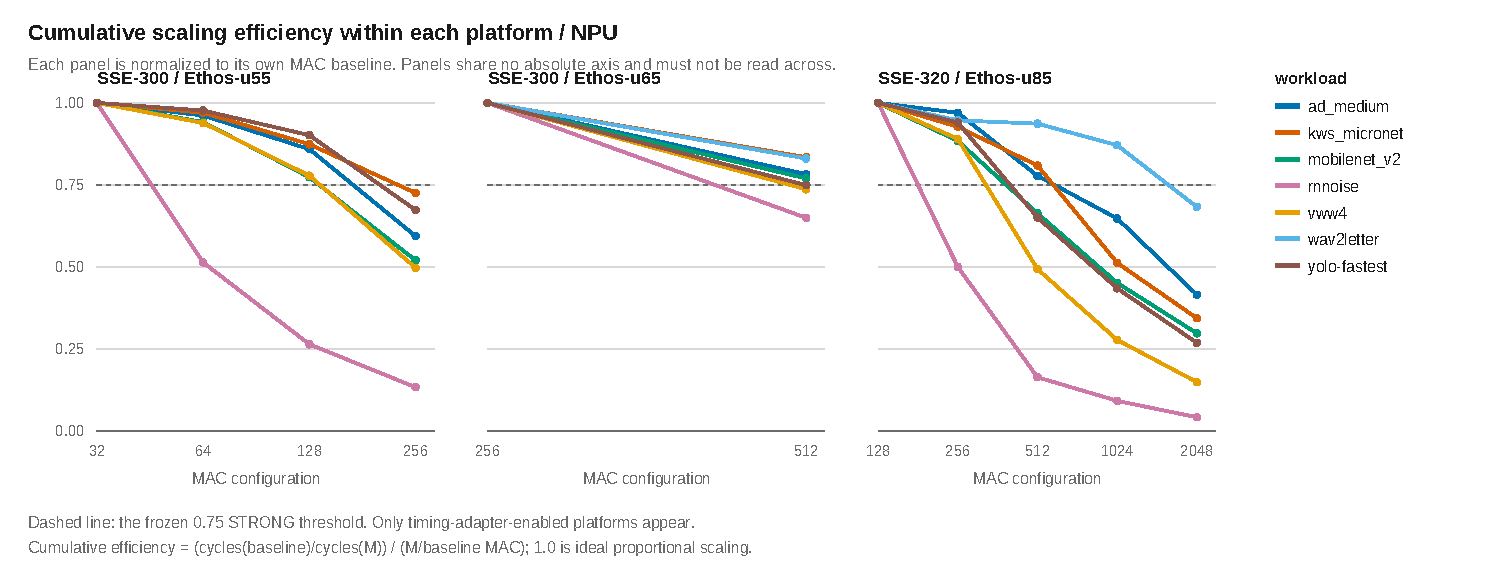
\includegraphics[width=\linewidth]{figures/fig1_mac_scaling.pdf}
  \Description{Cumulative scaling efficiency within each platform and NPU. Each panel is normalized to its own MAC baseline; the panels share no absolute axis and must not be read across as a cross-generation performance comparison. Dashed line: the frozen 0.75 \texttt{STRONG} threshold.}
  \caption{Cumulative scaling efficiency, timing-adapter-enabled platforms only. Within-platform comparison only.}
  \label{fig:1}
\end{figure}
The single observed saturation point is the entry point for Section~\ref{sec:7}.

\subsection{Compiler estimates versus simulated observation}\label{sec:4.2}
Over 20 comparable ladders, each series normalized independently: saturation classification agreed in 19/20, normalized speedup ordering agreed in 19/20 (Spearman \texttt{rho == 1.0}), while per-step incremental class agreement ranged from 4/4 down to 0/1.

\emph{Supported:} Vela preserves coarse scaling structure --- whether a configuration keeps scaling, and the ordering of normalized speedups --- but is less reliable for the class of an individual MAC step. \emph{Not established:} any accuracy, error percentage, or systematic bias of Vela against FVP cycles; no absolute error or calibration was computed, and the analysis contract rejects one.

\subsection{Workload ranking stability}\label{sec:4.3}
Over 55 configuration pairs: \texttt{rho == 1.0} in 31/55, minimum 0.9429, median 1.0000. Ordering is the portable quantity of this dataset; absolute cycles are not comparable across generations at all.

\subsection{Executability as a result (RQ1 boundary condition)}\label{sec:4.4}
All 133 capability cells compiled under Vela; \textbf{6 could not run}. The failures are homogeneous --- \texttt{wav2letter\_pruned\_int8} $\times$ Ethos-U55 $\times$ \texttt{Shared\_Sram} at MAC 32/64/128 --- and each reached a linker SRAM overflow after the deterministic minimum-increment arena retry, meaning the smallest arena that could clear the first allocation failure already did not fit. \texttt{EXECUTABILITY\_UNRESOLVED} was 0.

Classification: \textbf{system-level memory / deployability limitation}, not a U55 microarchitecture limit; MAC count, NPU, memory mode, and platform memory map are confounded in those six cells. Compiler acceptance does not establish deployability, and a missing cell is a result rather than a gap in collection.

\subsection{RQ1 statement}\label{sec:4.5}
\emph{Supported:} the generations and configurations differ primarily in normalized scaling behaviour, workload ordering, and deployability characteristics, rather than in directly comparable absolute cycle values. Concretely, across the three axes the question names: \textbf{deployability differed} --- six cells were non-executable, all \texttt{wav2letter\_pruned\_int8} $\times$ Ethos-U55 $\times$ \texttt{Shared\_Sram} (Section~\ref{sec:4.4}); \textbf{saturation differed} --- the only observed instance in the tested range is one Ethos-U85 ladder (Section~\ref{sec:4.1}); and \textbf{workload ordering did not differ}, remaining invariant across configurations (\texttt{rho == 1.0} in 31/55 pairs, minimum 0.9429, median 1.0000; Section~\ref{sec:4.3}). \emph{Not established:} any ``U85 is faster than U55'' statement --- Fast Models version skew and timing-adapter differences make absolute cross-generation comparison unsupportable on this data.

\section{Validity of the structural metrics across platform and timing conditions}\label{sec:5}
\textbf{This section answers no research question.} Section~\ref{sec:4}, 6 and 7 use normalized, ordinal and threshold metrics to compare configurations that share no absolute cycle axis; this section asks whether those metrics survive a change of host platform at all. It is a validity check on the instruments of the study, reported before the results that depend on it, and it is deliberately not numbered among RQ1--RQ4.

92 cells, 276 samples, all vector-exact; 39/39 artifacts reproduced their frozen hashes, so every comparison below is a same-NPU-artifact comparison. Zero artifact-identity failures and zero rule failures.

Ranking agreement means identical order \emph{and} Spearman \texttt{rho = 1.0} at that MAC point. The two classes are reported separately and are not combined into a single rate; per-metric agreement counts and their qualification are given together below.

\textbf{The only disagreements are eight scaling-class labels}, all in CLASS B, and every one is \texttt{PARTIAL} on the TA\_ON side and \texttt{STRONG} on the TA\_OFF side --- adjacent efficiencies of 0.64--0.75 against 0.77--0.86, i.e. crossings of the frozen 0.75 cut point in a single direction. No ranking, direction or saturation verdict changed anywhere.

In CLASS A the agreement is exact in a stronger sense: \textbf{14/14 tested cells had exactly identical canonical NPU cycles} on SSE-310 and SSE-315. Stated narrowly --- under the tested TA-OFF condition, changing from SSE-310 to SSE-315 produced no observable change in canonical NPU cycles for any of the 14 evaluated cells (\texttt{NO\_OBSERVED\_CYCLE\_DIFFERENCE\_UNDER\_TESTED\_TA\_OFF\_PAIR}). This observation does not establish that subsystem or Fast-Models differences are generally irrelevant, nor does it transfer to TA-ON conditions, which is \texttt{NOT\_EVALUABLE} here because no platform pair on this stack holds TA constant at TA\_ON.

All observed scaling-class disagreements occurred in comparisons where TA state also differed; they are \texttt{ASSOCIATED\_WITH} those comparisons and are not attributed to any one factor, because in CLASS B the subsystem, the Fast Models implementation and the TA state change together and remain \texttt{NOT\_SEPARATED}. What this does and does not license is discussed in Section~\ref{sec:8}.

Resulting qualification of the metrics, as categories rather than scores. This table is the metric hierarchy the rest of the paper relies on: a reader scanning results should not give a threshold class the same weight as an ordinal one.

\begin{center}\small
\begin{tabularx}{\linewidth}{LlrL}
\toprule
metric & tested universe & agreement & qualification \\
\midrule
workload ranking & 2 (A) + 8 (B) MAC points & 2/2, 8/8 & \texttt{ROBUST\_IN\_TESTED\_PAIRS} \\
MAC-step direction & 7 (A) + 32 (B) steps & 7/7, 32/32 & \texttt{ROBUST\_IN\_TESTED\_PAIRS} \\
saturation verdict & 7 (A) + 20 (B) ladders & 7/7, 20/20 & \texttt{ROBUST\_IN\_TESTED\_PAIRS} \\
normalized workload ordering & 2 (A) + 8 (B) MAC points & 2/2, 8/8 & \texttt{ROBUST\_IN\_TESTED\_PAIRS} \\
threshold scaling class & 7 (A) + 32 (B) steps & 7/7, \textbf{24/32} & \texttt{TA\_STATE\_SENSITIVE} \\
raw cross-platform cycles & --- & --- & \texttt{NOT\_COMPARABLE} \\
memory PMU counters & --- & --- & \texttt{GENERATION\_SPECIFIC\_NOT\_COMMON} \\
transfer of the CLASS A result to TA\_ON & --- & --- & \texttt{NOT\_EVALUABLE} \\
\bottomrule
\end{tabularx}
\end{center}
CLASS A and CLASS B counts are listed side by side. No aggregate robustness score is defined. Figure~\ref{fig:2} summarizes these agreement counts metric by metric, with the two classes drawn separately.

\begin{figure}[t]
  \centering
  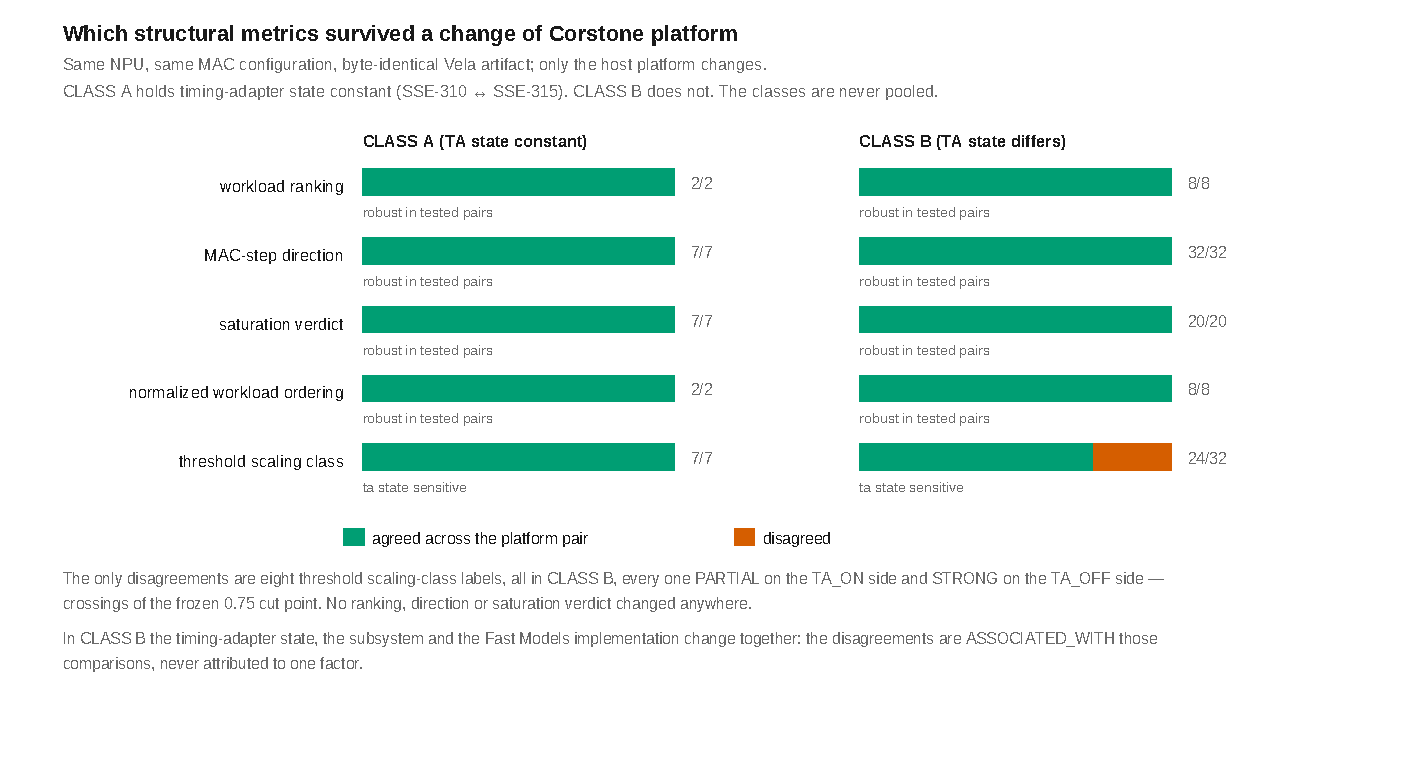
\includegraphics[width=\linewidth]{figures/fig2_platform_sensitivity.pdf}
  \Description{Agreement of each structural metric across a change of Corstone platform, CLASS A and CLASS B shown separately and never pooled. The only disagreements are eight threshold scaling-class labels, all in CLASS B.}
  \caption{Metric agreement across the tested platform pairs, same NPU and byte-identical Vela artifact. Not a platform performance comparison.}
  \label{fig:2}
\end{figure}
\section{Corstone-320 hardware validation (RQ3)}\label{sec:6}
The board contributes exactly one matrix cell: Corstone-320 / U85 @ 1024 MACs, seven workloads, three independent fresh boots --- \textbf{21 formal samples}.

\textbf{The protocol was corrected before any formal sample existed.} The registered 3 boots $\times$ 10 runs design was not executable: the stock runner performs exactly one inference per boot, and ``ten consecutive runs'' was a capability of a custom runner used in earlier campaigns. Since patching the artifact under test was not authorized, the protocol became 3 boots $\times$ 1 stock inference = 21 samples, recorded as a supersession. Canonical value per workload is \texttt{median(B1,B2,B3)}.

\textbf{Ranking preservation (primary).} Spearman \texttt{rho = 1.0}, \textbf{0 rank inversions} across all seven workloads: every workload holds the same position in the simulated and the physical ordering. The rank pairs are tabulated in Appendix~\ref{app:A}.

\textbf{Relative cost shape (secondary).} Each domain is normalized by its own geometric mean; Figure~\ref{fig:3} shows the two vectors and Appendix~\ref{app:A} gives the exact values.

The two vectors are presented side by side. \textbf{No aggregate deviation metric is computed}: \texttt{L1}, \texttt{L2}, RMSE, mean absolute percentage, and the board/FVP ratio were never preregistered, and selecting one with both vectors visible would be choosing a statistic to fit the result. Board repeatability is reported as the raw triplet plus median, with no spread statistic, for the same reason.

\begin{figure}[t]
  \centering
  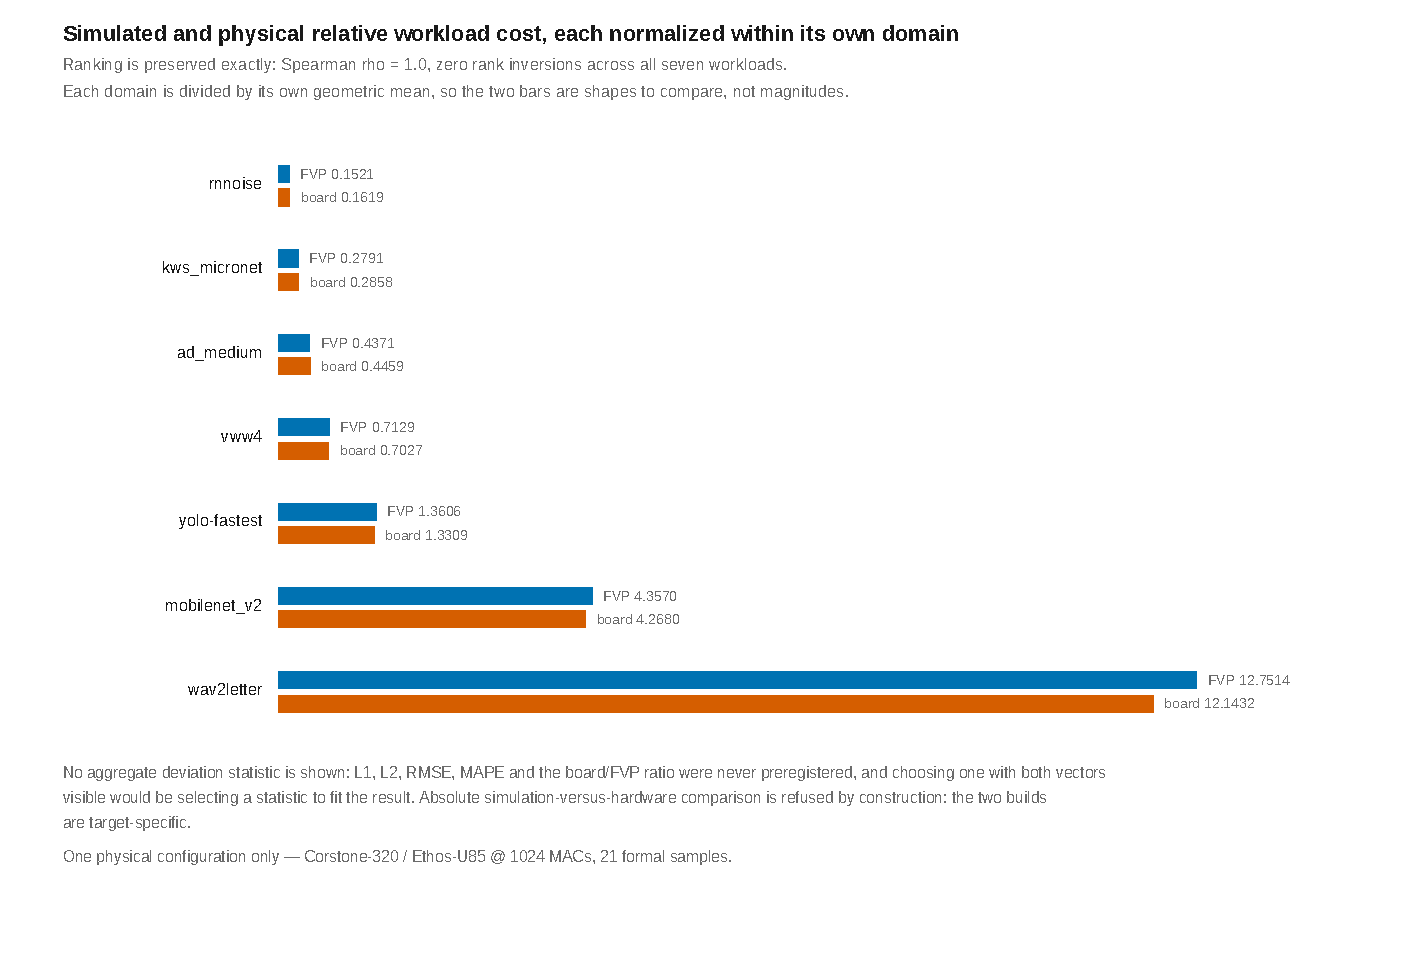
\includegraphics[width=\linewidth]{figures/fig3_board_relative_cost.pdf}
  \Description{Simulated and physical relative workload cost, each normalized within its own domain by its own geometric mean. Ranking is preserved exactly. No deviation, ratio or error statistic is shown.}
  \caption{Relative cost shape, FVP and board, independently normalized. The two vectors are shapes to compare, not magnitudes; absolute simulation-versus-hardware comparison is refused by construction.}
  \label{fig:3}
\end{figure}
Whether \texttt{rho = 1.0} constitutes strong validation is a judgement, not a threshold result: no pass/fail criterion was invented to declare it one. What this transfer does and does not establish is discussed in Section~\ref{sec:8}.

PMU cross-target status: \texttt{TOTAL}/\texttt{ACTIVE}/\texttt{IDLE} are present in both frozen sets but no board canonicalization across boots was preregistered; \texttt{SRAM\_*}/\texttt{EXT\_*} are board-collectable but absent from the frozen simulated records, hence \texttt{NOT\_EVALUABLE}. The frozen stages were not re-run to obtain them.

\section{Operator-level mechanism study: U85 256 $\rightarrow$ 512 (RQ4)}\label{sec:7}
\subsection{The anomaly and its scope}\label{sec:7.1}
Among the seven scaling workloads, exactly one becomes slower when the U85 doubles from 256 to 512 MACs: \texttt{rnnoise\_INT8}, 36,086 $\rightarrow$ 55,086 cycles (+19,000). Vela predicts improvement for every workload including this one, so the reversal is also a compiler-estimate/simulation disagreement point. \texttt{dnn\_s\_quantized}, on its separate track, also regresses (22,068 $\rightarrow$ 29,068).

A registered boundary condition: on this stack the 256 $\rightarrow$ 512 step also crosses a Vela system-config discontinuity (\texttt{SYS\_DRAM\_Low} at 128/256, \texttt{SYS\_DRAM\_Mid\_512} at 512). The mechanism study therefore compiled \textbf{both} bindings --- reproducing the sweep convention, and holding the system config fixed --- as a registered dual binding. For \texttt{rnnoise} and \texttt{dnn\_s} the two 512 bindings produce \textbf{byte-identical artifacts}, which excludes the system-config choice as the varying factor for exactly those workloads.

\subsection{Instrumentation}\label{sec:7.2}
Per-layer decomposition uses the post-compilation instrumentation path of Section~\ref{sec:3.4}, qualified as described in Section~\ref{sec:3.5}. Attribution uses the U85 interrupt-history mechanism: interrupts carry one-hot identifiers and the driver records the history mask consumed by each service, so when consecutive small operations merge into one service window the window's exact membership is recovered. Operations confined to unmixed windows receive exact cycles; operations sharing a window are \texttt{NOT\_SEPARATED} at operation granularity and are reported at operation-group granularity, which remains lossless.

Formal acquisition: 18 cells (6 workloads $\times$ 3 artifacts), clean and profiled arms, three fresh simulator processes per arm with full-vector exact equality, and profiled outputs bit-identical to the clean outputs on every profiled cell.

\subsection{The reversal is distributed, not localized}\label{sec:7.3}
For \texttt{rnnoise} at the sweep baseline, the +19,000-cycle reversal decomposes into \textbf{ten regressing groups of +1,000 to +4,030 cycles each}, with a single improving group ($-$1,000). The profiled groups sum to +19,060 rather than the +19,000 observed without instrumentation; the 60-cycle difference is the deterministic profiling-boundary residual of Section~\ref{sec:9.5}, and the two figures are reported separately rather than as one number. The largest contributor accounts for roughly a fifth of the whole-model delta. \textbf{No single pathological operation or group explains the reversal.} The regressing groups comprise small elementwise clusters (Add/Mul/Sub/Pack), small fully-connected operations, and Concat/Quantize --- the workload's abundant low-arithmetic operations rather than its few large matrix operations. Figure~\ref{fig:4} shows how that change is distributed across the groups, and places the +19,000 whole-model observed delta beside the +19,060 profiled-group sum so that the 60-cycle residual between the two measurement boundaries stays visible.

\begin{figure}[t]
  \centering
  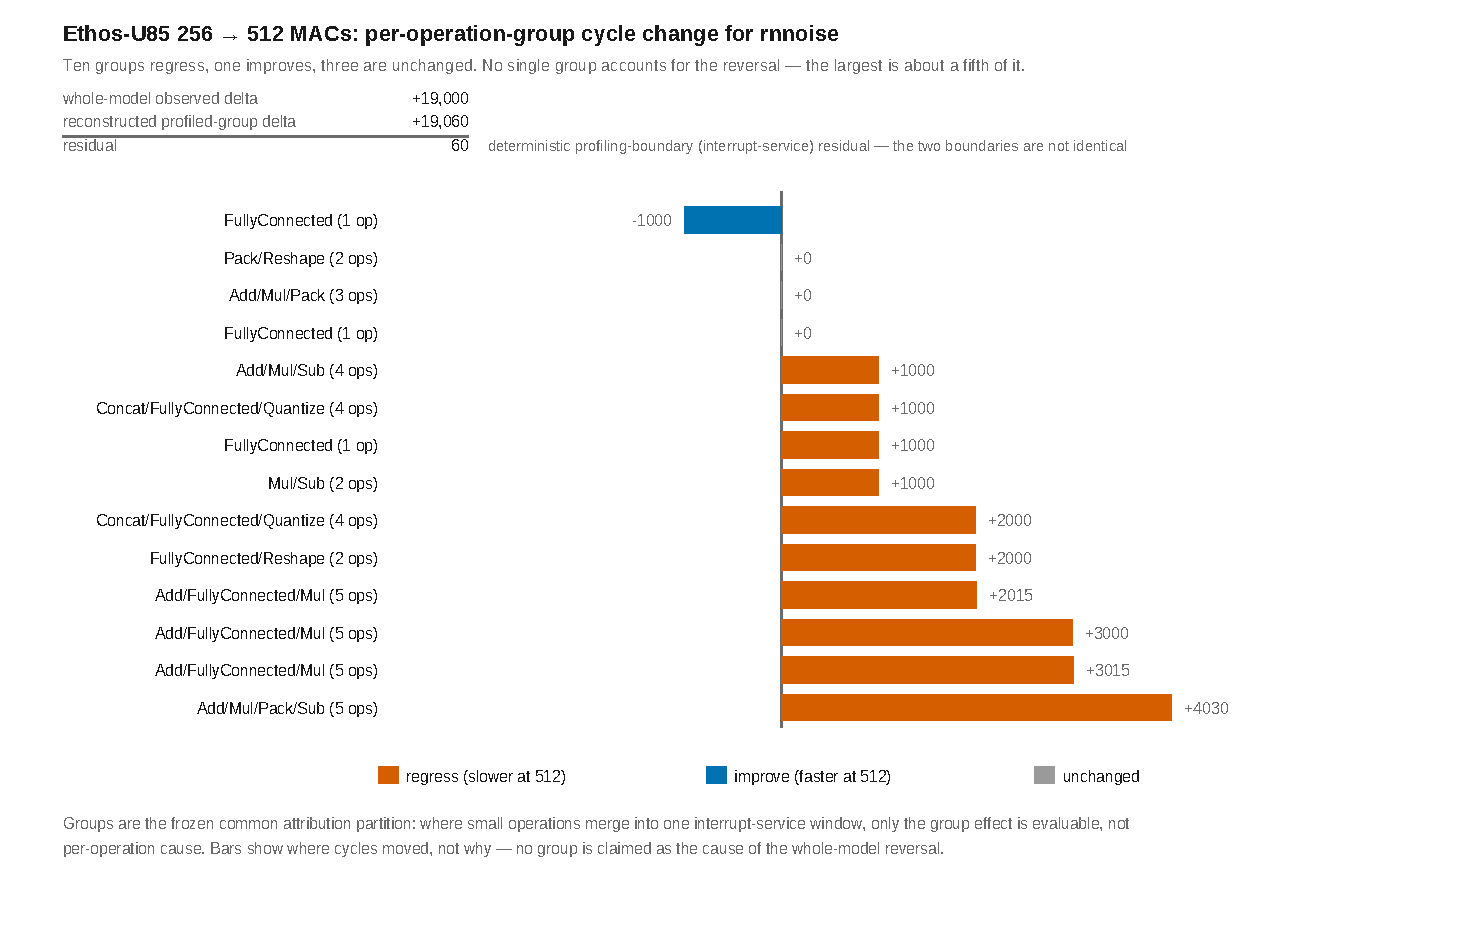
\includegraphics[width=\linewidth]{figures/fig4_u85_group_delta.pdf}
  \Description{Per-operation-group cycle change for rnnoise at the Ethos-U85 256 to 512 transition: ten groups regress, one improves, three are unchanged. The reconstructed profiled-group delta is +19,060 against a whole-model observed delta of +19,000, a residual of 60 cycles. Bars show where cycles moved, not why.}
  \caption{Distribution of the reversal across the frozen 14-group common attribution partition. The \textbf{whole-model observed delta is +19,000} cycles (Section~\ref{sec:7.1}); the \textbf{reconstructed profiled-group delta is +19,060}, and the \textbf{60-cycle residual} is the deterministic profiling-boundary (interrupt-service) residual described in Section~\ref{sec:9.5} --- the two measurement boundaries are not identical and the figure does not treat them as one. No group is claimed as the cause of the whole-model change; inside a merged interrupt-service window only the group effect is evaluable.}
  \label{fig:4}
\end{figure}
Two further observations bound interpretation. First, \texttt{UBLOCK\_CHANGED} co-occurs with roughly 95 \% of operations in \textbf{every} direction class (41/43 regressing, 63/65 improving, 14/16 unchanged), and \texttt{BLOCK\_CONFIG\_CHANGED} is \emph{more} frequent among improving operations (92 \%) than regressing ones (63 \%). The 256 $\rightarrow$ 512 ublock transition is therefore associated with widespread operator-level change, but \textbf{ublock change alone does not distinguish improving from regressing operations}. Second, per-operator regressions also exist inside workloads whose whole-model result improves --- 19 regressing operations summing +31,015 in \texttt{vww4} against $-$56,000 of improvements, 21 summing +40,985 in \texttt{yolo} against $-$140,000.

\subsection{Robustness to memory configuration}\label{sec:7.4}
A capability audit of the memory configurations admitted three tuples on this stack (\texttt{Sram\_Only}, \texttt{Shared\_Sram}, \texttt{Dedicated\_Sram}); no Ethos-U85 Flash system configuration exists, so that prior-study tuple is \texttt{NOT\_SUPPORTED}.

\textbf{Whole-model direction is invariant across all three; magnitude is not:}

\begin{center}\small
\begin{tabular}{lrrr}
\toprule
workload & Sram\_Only & Shared\_Sram & Dedicated\_Sram \\
\midrule
rnnoise & \textbf{+3,000} & \textbf{+15,000} & \textbf{+19,000} \\
dnn\_s & \textbf{+2,000} & \textbf{+6,000} & \textbf{+7,000} \\
vww4 & $-$83,000 & $-$32,000 & $-$28,000 \\
yolo & $-$288,000 & $-$244,000 & $-$225,000 \\
\bottomrule
\end{tabular}
\end{center}
No configuration removes a reversal and none creates one. Because every memory mode compiles to a \textbf{different artifact}, the contribution of memory-system behaviour versus compiler-generated program change remains \texttt{NOT\_SEPARATED}.

\textbf{The same logical groups regress in every configuration.} Cross-memory decomposition of \texttt{rnnoise} (12 profiled cells, one common attribution partition) shows 27 of 29 groups direction-consistent across all three modes and \textbf{zero direction flips}, with the recurring clusters scaling monotonically:

\begin{quote}\small\begin{verbatim}
Add/FC/Mul/Pack        +1k -> +4k -> +7k     (Sram_Only -> Shared_Sram -> Dedicated_Sram)
Add/FC/Mul/Pack        +1k -> +5k -> +6k
Concat/FC/Quantize     +1k -> +3k -> +2k
\end{verbatim}\end{quote}
Figure~\ref{fig:5} shows those group deltas side by side across the three configurations, where the magnitudes move and the directions do not.

\begin{figure}[t]
  \centering
  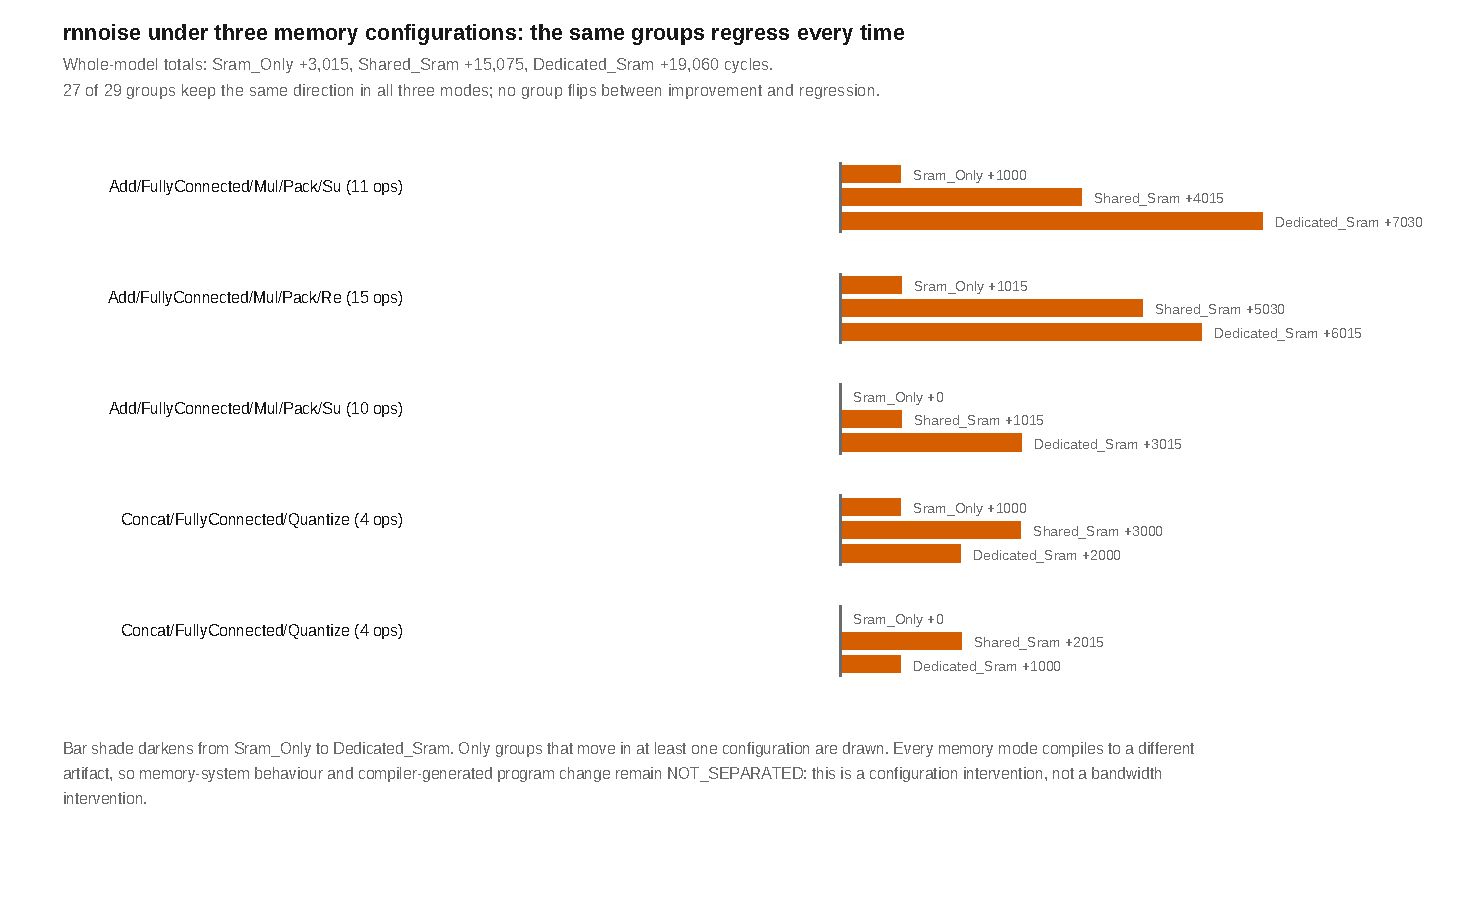
\includegraphics[width=\linewidth]{figures/fig5_u85_memory_robustness.pdf}
  \Description{rnnoise operation-group deltas under Sram\_Only, Shared\_Sram and Dedicated\_Sram. The same groups regress in every configuration; magnitude changes, direction does not.}
  \caption{Cross-memory robustness of the regressing groups. Every mode compiles to a different artifact, so memory-system behaviour and compiler-generated program change remain \texttt{NOT\_SEPARATED}; this is a configuration intervention, not a bandwidth intervention.}
  \label{fig:5}
\end{figure}
The control workload \texttt{vww4} behaves differently and instructively: its whole-model result improves in every mode, yet local regressions persist in every mode (a single Conv2D at +2,000 in all three), and \textbf{11 of 33 groups are direction-sensitive} to the memory configuration --- most prominently a 33-operation cascade group moving from $-$35,000 (Sram\_Only) through $-$2,120 (Shared\_Sram) to \textbf{+7,015 (Dedicated\_Sram)}. The same logical group crosses from improvement into regression as the configuration changes. Per-operation cause inside such multi-operation windows is \texttt{NOT\_EVALUABLE}; only the group effect is evaluable, and claims are phrased as ``the multi-operation execution group containing \ldots{}'' accordingly.

\subsection{Cross-backend instrumentation bridge (U65)}\label{sec:7.5}
Because the historical U55/U65 per-layer method and the U85 method are different instrumentation backends (Section~\ref{sec:3.4}), we tested whether they implement the same measurement boundary --- on Ethos-U65, with \textbf{both methods applied to the same clean program}, so that no compiler-backend difference enters the comparison.

Structural result: zero-modification round trips byte-identical; stripping the interrupt contribution from either method reconstructs the clean stream exactly; boundary positions and identifiers match exactly (14/14 and 46/46); and the two independently produced instrumented streams are \textbf{byte-identical}.

Runtime result across two cells, three fresh processes per arm: outputs identical to each other and to the clean run; segmentation and ordering identical; per-segment and summed \texttt{CYCLE} and \texttt{ACTIVE} \textbf{exact}; AXI beat fields \textbf{not exact} ($\leq$ 8 beats per segment, $\leq$ 7 in whole-profile sums).

Because exact equality of the complete PMU vector was a frozen preregistered criterion, the overall verdict is **\texttt{NOT\_EQUIVALENT}**; that criterion is not redefined post hoc. Component-level conclusions:

\begin{quote}\small\begin{verbatim}
STRUCTURAL_EQUIVALENCE          ESTABLISHED
SEMANTIC_BOUNDARY_EQUIVALENCE   ESTABLISHED
ATTRIBUTION_EQUIVALENCE         ESTABLISHED
CYCLE_DOMAIN_EQUIVALENCE        ESTABLISHED
ACTIVE_DOMAIN_EQUIVALENCE       ESTABLISHED
AXI_BEAT_EXACT_EQUIVALENCE      NOT_ESTABLISHED
\end{verbatim}\end{quote}
The beat residual \textbf{cannot be attributed specifically to the instrumentation backend}: an uninstrumented re-containerization control, with zero interrupts inserted, reproduced comparable beat-level and $\pm$1-cycle variation. The residual is \texttt{ASSOCIATED\_WITH} container re-serialization; no mechanism is claimed as uniquely proven.

Consequently the bridge permits cross-backend comparison of \textbf{execution boundaries, attribution, and cycle-domain mechanism observations} under the tested U65 conditions. It does \textbf{not} qualify exact cross-backend memory-traffic comparison, and it does not establish cross-generation PMU-event equivalence, which the event audit treats separately.

\subsection{Summary of the mechanism measurements}\label{sec:7.6}
Three measurement outcomes close this section.

\begin{enumerate}
  \item The 256 $\rightarrow$ 512 transition produces \textbf{heterogeneous operator-level cost changes in both directions}: some operations gain from the larger MAC array, others lose, and the whole-model outcome is the aggregate of that balance rather than the behaviour of any single group.
  \item \texttt{UBLOCK\_CHANGED} accompanies roughly 95 \% of operations in \textbf{every} direction class, so it does not discriminate regressing operations from improving ones.
  \item Memory configuration modulates the magnitude of the group deltas and, for some groups, their direction, while every memory mode compiles to a different artifact.
\end{enumerate}
The framing these outcomes support, and the single-factor account they retire, are in Section~\ref{sec:8}.

\section{Discussion}\label{sec:8}
\textbf{The compiler predicts shape better than steps.} Vela matched saturation classification in 19/20 ladders and preserved speedup ordering in 19/20, while per-step class agreement ranged 4/4 to 0/1. Pruning a design space on predicted \emph{trend} is supported by this data; ranking candidates on predicted \emph{magnitude} is not.

\textbf{Ordering is the portable quantity.} Workload ranking was stable across simulated configurations (\texttt{rho} median 1.0000) and transferred to hardware with zero inversions, while absolute cycles are not comparable across generations at all. This also explains why a single-cell board campaign can be decisive: ranking preservation remains comparable even when MAC scaling and absolute cycles are not.

\textbf{Compilation is not deployment.} All 133 cells compiled; 6 could not run. For the largest workload, executability --- not throughput --- was the binding constraint, and a scaling table must be read with missing cells as results.

\textbf{More hardware is not monotonically faster, and the reason is distributed.} The one reversal in the sweep survives every memory configuration tested and arises repeatedly from the same operation groups, yet no single group or single compiler-visible transition accounts for it. For practitioners, the actionable form is that a MAC upgrade must be validated per workload: models dominated by many small, low-arithmetic operations can lose more on those operations than they gain elsewhere, and a compiler estimate will not necessarily reveal it --- Vela predicted improvement for the one workload that regressed.

\textbf{What the mechanism evidence supports, and what it retires.} The evidence supports one framing and retires another. \emph{Supported --- emergence from heterogeneous local changes.} Whether a whole model improves or regresses across a MAC transition is the aggregate outcome of a balance between operation groups that gain and operation groups that lose:

\begin{quote}\small\begin{verbatim}
              U85 256 -> 512 transition
                        v
      heterogeneous operator-level cost changes
                        v
        +---------------+---------------+
  persistent regressions          config-sensitive
  (same groups, every mode)       local changes
        |                               |
     rnnoise                          vww4
  regressions outweigh gains    gains still outweigh regressions
        v                               v
  whole-model REGRESSION          whole-model IMPROVEMENT
\end{verbatim}\end{quote}
\emph{Retired --- the single-factor ublock account.} ``Ublock enlargement causes the regression'' is not supported: ublock change is a \textasciitilde{}95 \% background rate in every direction class. What the small-operation composition of the regressing clusters licenses is that the observations are \texttt{CONSISTENT\_WITH} a small-spatial / low-arithmetic-utilization account, while remaining \texttt{NOT\_SEPARATED} from the compiler-scheduling changes that accompany the same transition. Memory configuration modulates both magnitude and, for some groups, direction, but single-factor claims (``shared-SRAM contention causes\ldots{}'', ``bandwidth causes\ldots{}'') are unavailable: the memory-mode axis is a configuration intervention, not a bandwidth intervention, and every mode is a different artifact.

\textbf{What the board comparison establishes.} It establishes that \textbf{ordinal structure and relative cost shape transfer from the cycle model to this hardware configuration}, and nothing about absolute agreement. The two builds are target-specific --- FVP and FPGA binaries are not interchangeable for Corstone-320 --- so any absolute deviation would also include whatever those builds differ in, which is why no deviation statistic is reported at all.

\textbf{Which metrics transfer across platform and timing conditions.} The same-artifact validation turns a previously implicit assumption into a measured one. Ordinal and directional conclusions were preserved across the tested platform pairs, whereas threshold-based scaling classes were more sensitive to timing-model configuration. That yields a practical hierarchy: workload ordering, scaling direction, saturation verdicts and normalized ordering carried across every tested pair; a class label defined by a fixed efficiency cut point did not, because values sitting near the cut point can cross it; and raw cross-platform cycles remain outside the comparable set entirely. Readers reproducing this kind of study on a different simulator stack should expect the ordinal layer to travel and the thresholded layer to need re-qualification. The eight disagreements license a scoped statement and no more: they occurred only where timing-adapter state also differed, and since the subsystem, the Fast Models implementation and the adapter state change together in those comparisons, no one of the three can be named as the factor responsible.

\textbf{Measurement methodology results.} Four are reusable beyond this study. (i) A simulator's timing-adapter configuration can silently change what is being measured: the same NPU artifact exhibited a large cycle difference --- a byte-identical command stream measured \textasciitilde{}4$\times$ apart --- between the SSE-300 and SSE-310 conditions, and nothing in the cycle counts signalled it. Because timing-adapter state, subsystem and Fast Models timing implementation differ together across that pair, the magnitude cannot be attributed to the timing adapter alone; the three contributions are \texttt{NOT\_SEPARATED} (Section~\ref{sec:9.2}). The observation is therefore treated as a methodology warning against raw cross-platform cycle comparison, not as a performance result. (ii) A compiler backend change can silently change which program is instrumented: the default \texttt{regor} routing means legacy-core instrumentation decomposes a different binary than the formal sweep executes --- which is why this paper separates the three paths explicitly. (iii) Firmware embedding its own build timestamp is not byte-reproducible until the build epoch is pinned to source identity. (iv) Executability classification belongs before the sweep: the formal sample count could not be fixed until the filter ran (399 assumed; 222 actual).

\section{Limitations}\label{sec:9}
Fourteen limitations are recorded, grouped here under six themes. The grouping changes their presentation only; none has been withdrawn or softened. Read as a whole they say something specific rather than something global: the ordinal and structural results of this paper are established, the threshold-based labels are established only under the timing conditions tested, and a small number of questions --- chiefly which of several co-varying factors produces an observed effect --- remain \textbf{not separable} with this evidence and are marked as such wherever they arise.

\subsection{Simulation and timing-model validity}\label{sec:9.1}
\textbf{The timing adapter splits the matrix.} Only 11 of 19 configurations are benchmarking-valid; the 56 TA-OFF cells are capability and diagnostic evidence only. A claim retracted during this work: ``same NPU across different Corstone generations'' is not a clean platform isolation, because the two sides differ in adapter state --- a memory-constrained model against an unconstrained one.

\textbf{Determinism is exact, and that is the point.} \texttt{M1 == M2 == M3} held on 74/74 simulated cells, so the repetitions are not a statistical sample; no mean, median, or confidence interval is reported for them. Board repetitions are physical observations where equality is not required, and are reported as raw triplets with a median.

\textbf{Scope.} All simulated values are cycle-model observations on TA-enabled configurations with a stock single-inference runner; all board values are software-visible observations on one physical configuration. Workloads are the MLEK set --- representative of embedded ML, not exhaustive.

\subsection{Cross-platform and cross-generation comparability}\label{sec:9.2}
\textbf{Absolute cross-generation comparison is unsupportable.} Fast Models version skew and platform configuration differences confound it; comparisons are restricted to normalized scaling and ordinal ranking.

**\texttt{SSE-300 / U55@256} versus \texttt{U65@256} is a system-level configuration comparison**, not a microarchitecture result: the memory mode differs by NPU (\texttt{Shared\_Sram} versus \texttt{Dedicated\_Sram}), moving weights between SRAM and DRAM.

\textbf{Platform-sensitivity validation bounds.} The validation covers U55 and U65 on the platform pairs this stack supports; three bounds follow. There is \textbf{no same-platform U65-versus-U85 controlled pair}, so cross-generation statements involving U85 rest on structural metrics rather than a controlled substrate. There is \textbf{no TA\_ON cross-FVP control pair}, so the CLASS A result exists only under TA\_OFF and its transfer to TA\_ON is \texttt{NOT\_EVALUABLE}. In CLASS B the timing-adapter state, the subsystem and the Fast Models implementation change together, so their contributions are \texttt{NOT\_SEPARATED}; the eight class disagreements are reported as associated with those comparisons, never as caused by any one of the three.

\subsection{Compiler and instrumentation paths}\label{sec:9.3}
\textbf{Instrumentation-bridge bounds.} The overall U65 bridge verdict is \texttt{NOT\_EQUIVALENT} under its preregistered full-PMU-vector criterion. Execution boundaries, attribution, and the cycle and active-cycle domains are established as equivalent; exact cross-backend memory-traffic comparison is not qualified, and the bridge does not establish cross-generation PMU-event equivalence. It was run at U65-256 on two cells with a forced-legacy clean program; other command structures were not exercised. Historical U55/U65 per-layer data is therefore usable for cycle-domain mechanism observations on its own program, and is not an exact decomposition of the frozen regor formal executables.

\textbf{A withdrawn auxiliary observation.} An earlier auxiliary record reported that an FVP accepted an unsupported \texttt{num\_macs} value, and was used to argue that the model range-checks bounds without validating the discrete set. The exact probe invocation was not archived, the observation could not be reproduced under the same Fast Models build during the X0 capability audit (three invocation styles all reject, and the model enumerates the legal set in its own error), and it is classified \texttt{NOT\_REPRODUCIBLE} / \texttt{NOT\_LOAD\_BEARING}. No argument in this paper rests on it; Section~\ref{sec:3.1} states the authority rule directly instead.

\subsection{PMU and runner-output semantic coverage}\label{sec:9.4}
\textbf{PMU semantics are generation-conditional.} Only \texttt{CYCLE}, \texttt{NPU\_IDLE}, and \texttt{CC\_STALLED\_ON\_BLOCKDEP} were verified as common-semantics across generations; of 22 shared event names, 18 differ in ordinal, so event numbers never cross a generation boundary. \texttt{CC\_STALLED\_ON\_BLOCKDEP} cross-generation and the U85 \texttt{EXT*}/\texttt{SRAM*} family were \texttt{NOT\_EVALUABLE} --- absences in what the stock runner prints, and obtaining them would break the stock-runner contract under which every formal measurement was taken. U85 stall-family events remain \texttt{SEMANTICS\_UNVERIFIED} and were never collected, so stall-based causal attribution is \texttt{NOT\_EVALUABLE} throughout Section~\ref{sec:7}.

\textbf{The inference-count check is a completion check.} The stock runner prints \texttt{Total number of inferences: 1} as a string literal, not a counter; requiring it verifies that execution reached post-inference code, and must not be described as counting inferences.

\subsection{Causal identifiability}\label{sec:9.5}
\textbf{Mechanism-study attribution bounds.} Where small operations merge into one interrupt-service window, per-operation cause is \texttt{NOT\_EVALUABLE} and only the operation-group effect is evaluable --- for \texttt{rnnoise}, only 3 of 44 operations are individually separable, and its decomposition floor is the 14-group common partition. Each service boundary carries a small deterministic cycle residual, so group and whole-model sums agree within that residual. \texttt{dnn\_s} profiled arms are \texttt{NOT\_AVAILABLE}: its CPU-operator container uses a schema feature outside the audited rewrite subset, and the instrumentation failed closed rather than guessing.

\textbf{Memory-mode is not a bandwidth intervention.} It jointly moves weight placement, arena headroom, compiler scheduling, and the generated command stream; all mode pairs are different artifacts.

\textbf{Hardware geometry versus compiler scheduling is not causally separated} anywhere in this work, and no claim in Section~\ref{sec:7} asserts otherwise.

\subsection{Physical-board scope}\label{sec:9.6}
\textbf{Board scope.} One physical configuration (U85 @ 1024) means no physical scaling validation is possible; simulation and board binaries are target-specific, so any absolute deviation would include build differences; board \texttt{SRAM\_*}/\texttt{EXT\_*} counters have no counterpart in the frozen simulated records. No aggregate deviation or repeatability-variability statistic is reported, because none was preregistered.

\section{Conclusion}\label{sec:10}
We set out to characterize what an embedded ML deployment toolchain actually supports across the configurations a practitioner must choose between, and to be explicit about which comparisons the resulting evidence cannot carry.

\textbf{MAC scaling is workload-dependent and frequently sub-linear (RQ2).} Of 53 adjacent MAC transitions, 28 retained at least 75 \% efficiency and 23 fell between 50 \% and 75 \%; saturation appeared in one of 21 ladders within the tested range. More MAC capacity generally helps, and it generally helps less than proportionally, by an amount that depends on the workload rather than on a common saturation point.

\textbf{Structural conclusions travel better than thresholded labels (RQ1).} Across a same-artifact study over the supported Corstone FVPs, workload ranking, MAC-step direction, saturation verdict and normalized ordering were preserved in every tested pair, while the threshold-based efficiency class disagreed in 8 of 32 CLASS B steps --- all of them crossings of the frozen 0.75 cut point in one direction. The configurations therefore differ in normalized scaling behaviour, in deployability, and not in any directly comparable absolute cycle value: deployability differed (six non-executable cells), saturation differed (one U85 ladder), and workload ordering did not differ at all.

\textbf{The one non-monotonic boundary is distributed, not localized (RQ4).} Direct operation-group profiling of the Ethos-U85 256 $\rightarrow$ 512 transition shows the +19,060-cycle \texttt{rnnoise} reversal spread across ten regressing groups against one improving group, the largest about a fifth of the whole; the same groups regress under every memory configuration tested while their magnitudes change. A compiler-visible ublock change accompanies roughly 95 \% of operations in every direction class, so it does not discriminate regressing operations from improving ones, and no single group or single compiler-visible transition accounts for the reversal. Which of the co-varying factors produces it remains \texttt{NOT\_SEPARATED}.

\textbf{The three kinds of number are not interchangeable (RQ2, RQ3).} A Vela estimate, an FVP observation and a physical observation play different evidentiary roles here and are never placed on one axis. Vela preserved coarse structure --- saturation classification and normalized speedup ordering agreed in 19 of 20 ladders --- while per-step class agreement ranged from 4/4 to 0/1, so pruning a design space on predicted trend is supported by this data and ranking candidates on predicted magnitude is not.

\textbf{Physical validation establishes order, not timing accuracy (RQ3).} At the one configuration the hardware makes available --- Corstone-320 / Ethos-U85 @ 1024 MACs, 21 formal samples --- workload ranking was preserved exactly, with zero inversions, and the independently normalized relative-cost vectors have the same shape. This is evidence that ordinal structure transfers from the cycle model to this hardware point. It is not evidence about absolute simulator timing accuracy, which the target-specific builds make unavailable and which no result here depends on.

Two limits bound all of the above and are stated in full in Section~\ref{sec:9}: the comparisons rest on cycle-model observations under an enabled timing adapter with a stock single-inference runner, and wherever several factors change together --- timing-adapter state with subsystem and Fast Models implementation, memory mode with the compiled artifact, hardware geometry with compiler scheduling --- the contributions are reported as associated and never as separated.

The practical form of the result is short. A MAC upgrade must be validated per workload, because a model dominated by many small, low-arithmetic operations can lose more on those operations than it gains elsewhere, and the compiler estimate will not necessarily reveal it: Vela predicted improvement for the one workload that regressed.

\bibliographystyle{ACM-Reference-Format}
\bibliography{references}
\appendix
\section{Exact values behind the board validation}\label{app:A}
Reproduced from \texttt{docs/paper/analysis/board\_rq3/} so that the numbers behind Section~\ref{sec:6} and Figure~\ref{fig:3} remain available without re-running the frozen analysis. Corstone-320 / Ethos-U85 @ 1024 MACs, 21 formal samples, canonical value per workload \texttt{median(B1,B2,B3)}.

\textbf{A.1 Rank preservation.}

\begin{center}\small
\begin{tabularx}{\linewidth}{Lll}
\toprule
workload & FVP rank & board rank \\
\midrule
\texttt{rnnoise\_INT8} & 1 & 1 \\
\texttt{kws\_micronet\_m} & 2 & 2 \\
\texttt{ad\_medium\_int8} & 3 & 3 \\
\texttt{vww4\_128\_128\_INT8} & 4 & 4 \\
\texttt{yolo-fastest\_192\_face\_v4} & 5 & 5 \\
\texttt{mobilenet\_v2\_1.0\_224\_INT8} & 6 & 6 \\
\texttt{wav2letter\_pruned\_int8} & 7 & 7 \\
\bottomrule
\end{tabularx}
\end{center}
\textbf{A.2 Independently normalized relative cost.} Each domain is divided by its own geometric mean. The two columns are shapes to compare, not magnitudes: no ratio, difference, or error between them is computed anywhere in this paper.

\begin{center}\small
\begin{tabularx}{\linewidth}{Lll}
\toprule
workload & FVP normalized & board normalized \\
\midrule
\texttt{rnnoise\_INT8} & 0.1521 & 0.1619 \\
\texttt{kws\_micronet\_m} & 0.2791 & 0.2858 \\
\texttt{ad\_medium\_int8} & 0.4371 & 0.4459 \\
\texttt{vww4\_128\_128\_INT8} & 0.7129 & 0.7027 \\
\texttt{yolo-fastest\_192\_face\_v4} & 1.3606 & 1.3309 \\
\texttt{mobilenet\_v2\_1.0\_224\_INT8} & 4.3570 & 4.2680 \\
\texttt{wav2letter\_pruned\_int8} & 12.7514 & 12.1432 \\
\bottomrule
\end{tabularx}
\end{center}
\section{Provenance and procedure}\label{app:B}
Every formal cell carries an identity chain: model SHA $\rightarrow$ Vela artifact SHA $\rightarrow$ generated model-source body SHA $\rightarrow$ linked executable SHA $\rightarrow$ execution. Builds are byte-reproducible after pinning \texttt{SOURCE\_DATE\_EPOCH} to the source-tree commit timestamp --- necessary because the firmware embeds \texttt{\_\_DATE\_\_}/\texttt{\_\_TIME\_\_}, which made every binary unique until pinned.

Simulated cells use one discarded warm-up inference and three deterministic runs required to be \textbf{exactly equal}; disagreement is a hard stop, never an average, because a deterministic model disagreeing with itself indicates a harness fault. Board cells use three independent fresh boots. Invalid runs are discarded with a named reason and never down-weighted.

Analysis plans were frozen before the data they read, applied exactly once, and amended only by recorded supersession. Analyzers carry mutation tests proving each rejection rule can fire.


\end{document}
